	\documentclass[14pt]{extreport}
\usepackage{extsizes}
	\usepackage[frenchb]{babel}
	\usepackage[utf8]{inputenc}  
	\usepackage[T1]{fontenc}
	\usepackage{amssymb}
	\usepackage[mathscr]{euscript}
	\usepackage{stmaryrd}
	\usepackage{amsmath}
	\usepackage{tikz}
\usepackage{eurosym}
	\usepackage[all,cmtip]{xy}
	\usepackage{amsthm}
	\usepackage{varioref}
	\usetikzlibrary{patterns}
	\usepackage{float}
	\usepackage[ margin=1in]{geometry}
	\geometry{a4paper}
	\usepackage{lmodern}
	\usepackage{hyperref}
	\usepackage{array}
	\usepackage{easytable}
	 \usepackage{fancyhdr}\usepackage{longtable}

	\pagestyle{fancy}
	\theoremstyle{plain}
	\fancyfoot[C]{\empty} 
	\fancyhead[L]{Contrôle}
	\fancyhead[R]{20 mars 2024}
	
	
	\title{Contrôle chapitre 6}
	\date{}
	\begin{document}

\begin{center}{\Large Contrôle chapitre 6}\\ \textbf{Soignez votre présentation et votre rédaction.}\end{center}

\subsection*{Exercice 1 (4 points)}  % 4 points

Donner le périmètre des figures suivantes : \begin{enumerate}
\item Un carré dont un côté mesure $2$ cm. 
\item Un rectangle de longueur $3,2$ dm et de largeur $3,7$ dm. 
\item Un cercle de rayon $4$ cm (donner la valeur exacte, puis une valeur approchée au mm).
\item Le triangle ci-dessous. 
\begin{figure}[H]\center
\begin{tikzpicture}[scale = 3]
\draw (-0.5, 0) --  (3.5, 0) -- (0, 1.2) -- (-0.5, 0);
\draw[dashed] (0,0) -- (0,1.2); 
\draw [<->] (-0.5, -.1) -- (0, -.1); 
\draw [<->] (3.5, -.1) -- (0, -.1); 
\draw (-.25, -.2) node {$1,5$ cm};
\draw (1.65, -.2) node {$10,5$ cm};
%\draw [<->] (0.05, 0) -- (0.05, 1.2); 
\draw (0.29, .6) node {$3,6$ cm};
\draw (1.6, .8) node {$11,1$ cm};
\draw (-0.6, .6) node {$3,9$ cm};
\fill (0.1,0) -- (0.1, 0.1) -- (0, 0.1) -- (0,0);
\end{tikzpicture}
\end{figure}
\end{enumerate}

\subsection*{Exercice 2 (4 points)}

Calculer la longueur de la clôture nécessaire pour entourer le champ suivant (les longueurs sont en mètres).
\[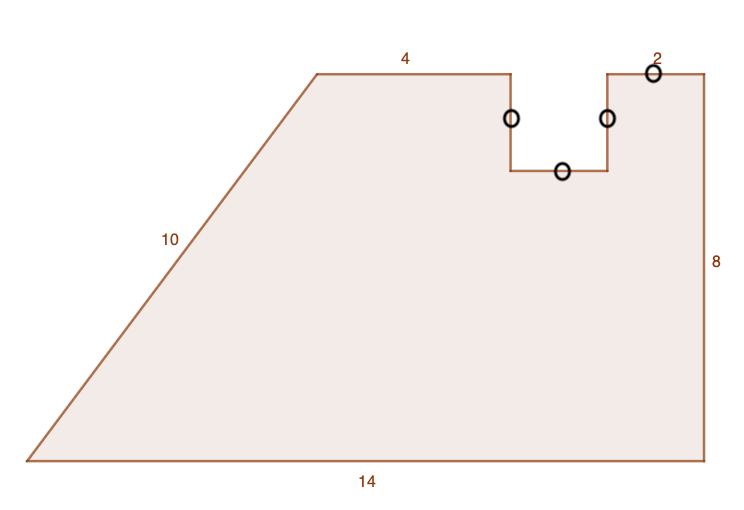
\includegraphics[scale=.5]{Exo1}\]



\newpage

\subsection*{Exercice 3 (5 points)}
On considère les deux figures suivantes : 

\begin{figure}[H]
\center 
\begin{tikzpicture}[scale =1.3]
\draw (-2, 0) -- (2, 0) arc (0: 180 :2);
\draw (-2, 0) -- (2, 0) arc (0: 180 :2);
\draw[<->] (-2, -.2) -- (2, -.2); 
\draw (0, -.5) node {$4\ cm$};
\draw[white](0,-1)--(3,-1);
\end{tikzpicture}
\begin{tikzpicture}[scale =1.3]
\draw[dashed](-2, 0) -- (2, 0);
\draw(2,0) arc (0: 180 :2) arc (180:360: 1) arc(180:0:1);
\draw(2,0) arc (0: 180 :2) arc (180:360: 1) arc(180:0:1);
\draw[<->] (2, -.2) -- (0, -.2); 
\draw (1, -.5) node {$2\ cm$};
\end{tikzpicture}
\end{figure} 
\begin{enumerate}
\item Calculer le périmètre des deux figures. Donnez d'abord une valeur exacte faisant apparaître $\pi$, puis une valeur approchée au millimètre.

\item Laquelle des figures a le plus grand périmètre ? 
\end{enumerate} 

 \subsection*{Exercice 4 (6 points)}
 
 Le plan ci-dessous représente une pièce autour de laquelle on veut poser des plinthes. 
\begin{center} 
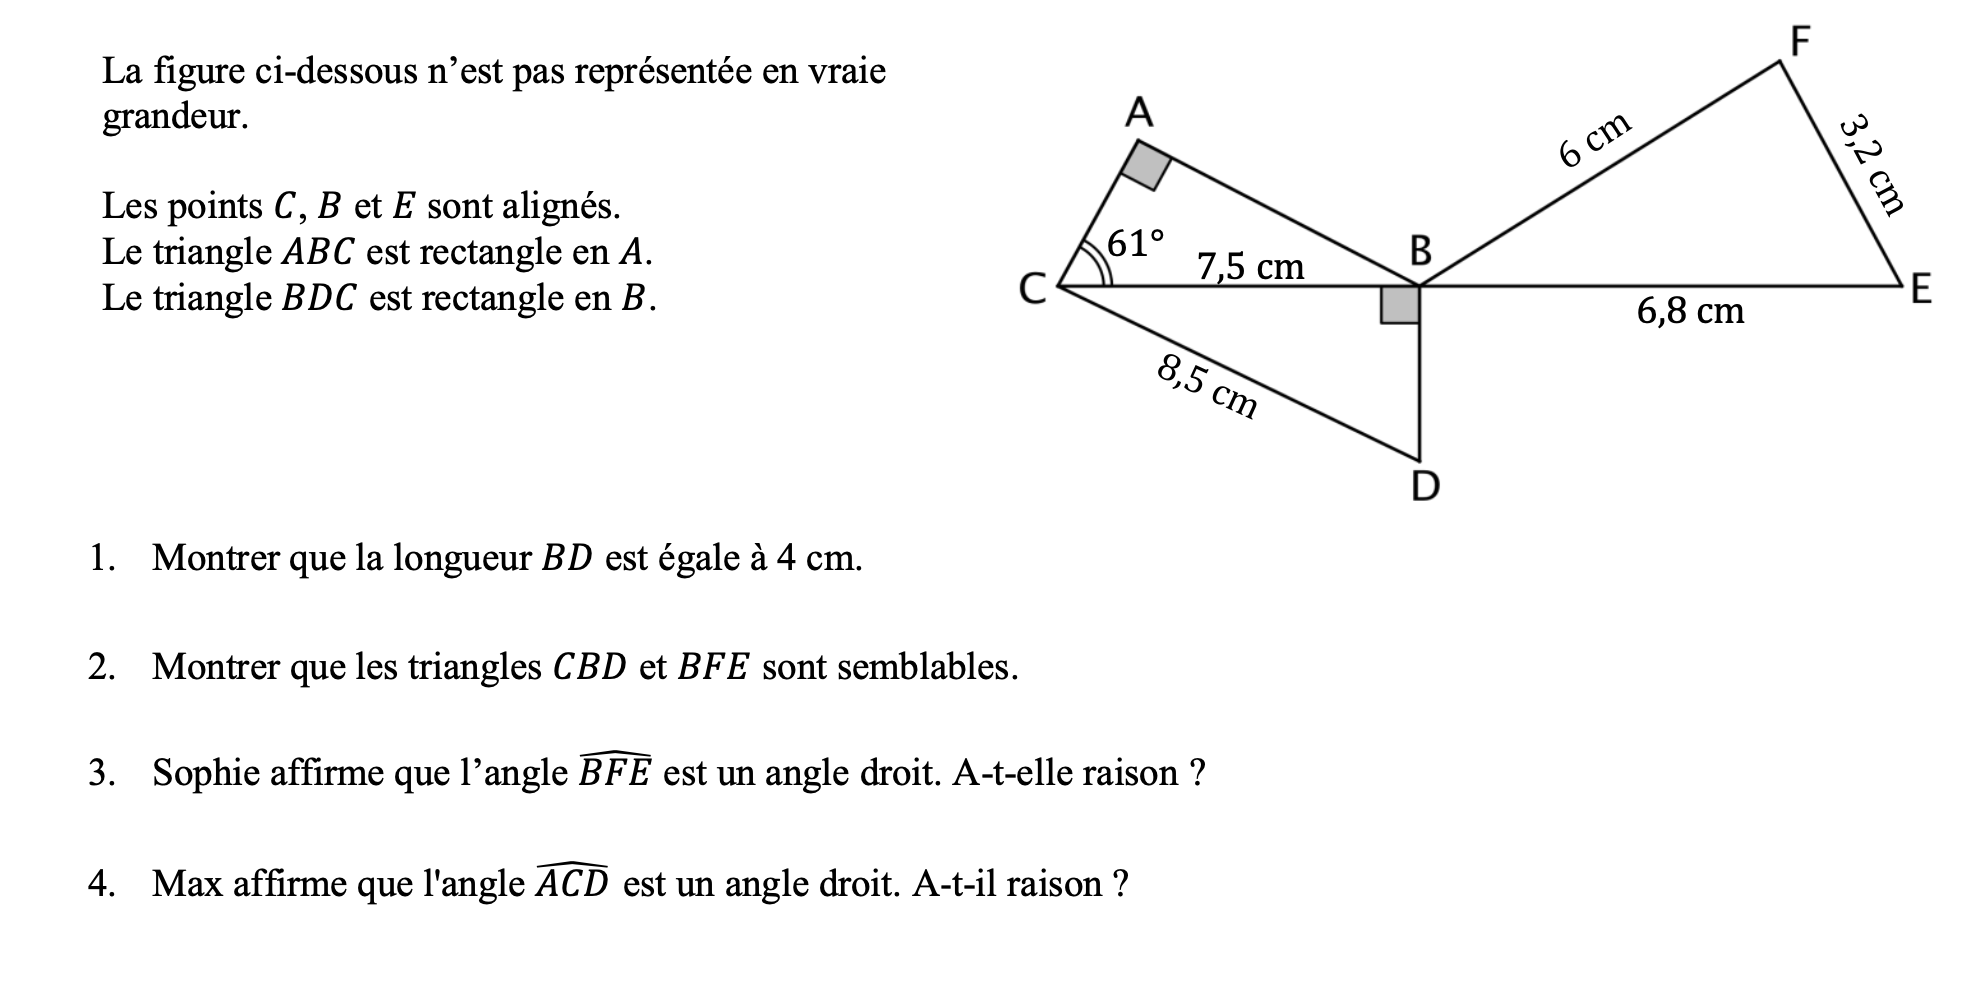
\includegraphics[scale=1.15]{Exo3}
\end{center}
\begin{enumerate}
\item Calculez la longueur du demi-cercle situé en haut de la figure. Donnez la valeur exacte, puis une valeur arrondie au décimètre. 
\item Déterminez la longueur de plinthes nécessaire pour entourer toute la pièce (sauf la porte).
\item Si un mètre de plinthes coûte $17$ euros, combien devra-t-on payer au total ? 
\end{enumerate}

\end{document}